\documentclass[a4paper]{article}

%% Language and font encodings
\usepackage[english]{babel}
\usepackage{graphicx}
\usepackage[T1]{fontenc}
\usepackage[utf8]{inputenc}

%% Sets page size and margins
\usepackage[a4paper,top=3cm,bottom=3cm,left=3cm,right=3cm,marginparwidth=1.75cm]{geometry}
%% To use hyperlinks
\usepackage{hyperref}
%% To use colors
\usepackage[usenames,dvipsnames,svgnames,table]{xcolor}

%%To use maths
\usepackage{amssymb}
\usepackage{amsmath}
\usepackage{mathtools}

\title{\textbf{Aprendizagem Automática} \\
\large Assignment 1 - Classifiers}

\author{Andrea Mascaretti N52222\and Daniel Pimenta N45404}

\begin{document}
\maketitle

\begin{abstract}
The main goal of this assignment was the parameterization, fitting and comparation of Logistic Regression,
 K-nearest Neighbours and Naive Bayes classifiers.\\ 
The data set used was the banknote authentication which was obtained from the
 \hyperref['https://archive.ics.uci.edu/ml/datasets/banknote+authentication]{UCI machine learning repository}.\\
To achieve our goals we used the Spyder IDE with programming language Python 3.6 and some of its modules 
such as \textit{Panda} to load and manage our data, \textit{NumPy} which is the fundamental package for 
scientific computing with Python and was used for various mathematical calculations and managing multidimensional 
arrays, \textit{sklearn (scikit-learn)} which has efficient tools for data mining and data analysis used in our assignment 
to preprocess data (shuffle, standardize, split), fold our data into k stratified folds, calculate cross validation score and 
fit our data on Logistic Regression and K-nearest Neighbours classifiers. Another imported module was Matplotlib.Pyplot
 which provides a MATLAB-like plotting framework used to build the error plots. 
\end{abstract}

\section{Introduction}

WHAT WE INITIALLY HAD,\\
WHAT WAS ASKED TO DO,\\
HOW WE PLAN ON DOING IT\\

\section{Classifiers}

\subsection{Logistic Regression}

The logistic regression is a generalised linear model. Before considering
a more classic machine learning framework, we provide a brief introduction
to the main idea behind the model. 

The logistic regression is composed, as every linear model, of three
part:
\begin{itemize}
	\item A sequence of \textit{response variables} $Y_{1},\,\ldots,\,Y_{n}$.
	Such response variables are called random components. The main assumption
	we shall make regarding those variables is that they are all independent
	random variables. Moreover, each one of them will have a distribution
	from the exponential family. Bear in mind that we are not imposing
	that the various $Y_{i}$s are identically distributed.
	\item The \textit{systematic component} is our model. It is a function of
	some predictors (also known as regressors or covariates), linear in
	the parameter and related to the mean of $Y_{i}$.
	\item The \textit{link function} $g\left(\mu_{i}\right)$ will allow us
	to link the two components, allowing us to say that 
	\begin{equation}
	g\left(\mu_{i}\right)=\beta_{0}+\sum_{i=1}^{r}\beta_{i}x_{i}\label{eq:-3}
	\end{equation}
	where $\mu_{i}=\mathbb{E}\left[Y_{i}\right]$. In the machine learning
	framework, it is usually more common to consider the inverse of the
	link function.
\end{itemize}
In our model we will assume the following:
\begin{equation}
Y_{i}\overset{ind}{\sim}\mathsf{Bernoulli}\left(\pi_{i}\right)\label{eq:}
\end{equation}
and therefore we will have that 
\begin{equation}
\mathbb{E}\left[Y_{i}\right]=\pi_{i}.\label{eq:-1}
\end{equation}
Now, in this model we will assume a relationship between the logarithm
of the odds of success for $Y_{i}$ (the log odds or \textit{logit})
and the predictor $\mathbf{x}=\left(1,\,x_{1},\,\ldots,\,x_{r}\right)$.
Mathematically, this entails
\begin{equation}
\ln\left(\frac{\pi}{1-\pi}\right)=\mathbf{\beta^{\prime}\mathbf{x}}\label{eq:-6}
\end{equation}
and $\mathbf{\beta}=\left(\beta_{0},\,\ldots,\,\beta_{r}\right)$.

Rewriting in order to obtain the exponential family form we have
\begin{equation}
\pi^{y}\left(1-\pi\right)^{1-y}=\left(1-\pi\right)\exp\left\{ y\,\ln\left(\frac{\pi}{1-\pi}\right)\right\} ,\label{eq:-2}
\end{equation}
where the term $\ln\left(\frac{\pi}{1-\pi}\right)$ is the natural
parameter of the exponential family and shows why we will implement
the link function
\begin{equation}
g\left(\pi\right)=\ln\left(\frac{\pi}{1-\pi}\right).\label{eq:-4}
\end{equation}

Rewriting \ref{eq:-6}, we obtain
\begin{equation}
\pi\left(x\right)=\frac{\exp\left\{ \mathbf{\beta}^{\prime}\mathbf{x}\right\} }{1+\exp\left\{ \mathbf{\beta}^{\prime}\mathbf{x}\right\} }.\label{eq:-5}
\end{equation}

What we have written is equivalent to saying that 
\begin{equation}
\mathsf{p}\left(\mathcal{C}_{1}|\,\mathbf{x}\right)=\pi\left(\mathbf{x}\right)=\sigma\left(\mathbf{\beta}^{\prime}\mathbf{x}\right)\label{eq:-7}
\end{equation}
where $\sigma\left(\cdot\right)$ is the logistic sigmoid and $\mathcal{C}_{1}$
is to identify class $1$. Notice that it holds $\mathsf{p}\left(\mathcal{C}_{2}|\,\mathbf{x}\right)=1-\mathsf{p}\left(\mathcal{C}_{1}|\,\mathbf{x}\right)=1-\sigma\left(\mathbf{\beta}^{\prime}\mathbf{x}\right)$.

Suppose we are given a dataset $\left\{ \mathbf{x}_{i},\,y_{i}\right\} $
where now $y_{i}\in\left\{ -1,\,1\right\} $ and $\mathbf{x}_{i}\in\mathbb{R}^{r}$
for $i=1,\,\ldots,\,n$. Given our hypotheses, we can write the negative
log-likelihood function as
\begin{equation}
\sum_{i=1}^{n}\ln\left(1+\exp\left\{ -y_{i}\,\left(\mathbf{\beta}^{\prime}\mathbf{x}_{i}\right)\right\} \right).\label{eq:-8}
\end{equation}
To this term we added a $\mathsf{L2}$ penalization term to obtain
a more regularized result, preferring this to its $\mathsf{L1}$ version
as the latter usually provides sparser solutions and we were working
in an environment with only four covariates. This lead to the following
problem:
\begin{equation}
\underset{\mathbf{\beta}}{\min\,}f\left(\mathbf{\beta}\right)=\frac{1}{2}\mathbf{\beta}^{\prime}\mathbf{\beta}+C\,\sum_{i=1}^{n}\ln\left(1+\exp\left\{ -y_{i}\,\left(\mathbf{\beta}^{\prime}\mathbf{x}_{i}\right)\right\} \right),\label{eq:-9}
\end{equation}
where $C\,>\,0$ is a parameter that can be assigned in order to balance
the two terms. To tune it, we relied on a stratified 5-fold cross-validation
on the training set, picking the value that yielded the lowest value.
From a numerical point of view, the trust region Newton method built
in the $\mathsf{ScikitLearn}$ class for $\mathsf{L2}$-logistic regression
was used.

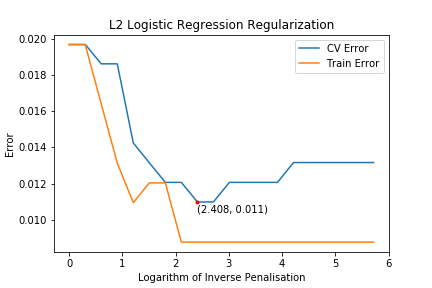
\includegraphics{Best C value - L2 Logistic Regression.png}

\subsection{k-Nearest Neighbours}

Suppose that we have some classes $\mathcal{C}_{k}$ such that each
class contains $N_{k}$ points and let $N=\sum_{k}N_{k}$ be the total
number of points. Let us suppose that we are also given a distance
function $\rho:\,\mathbb{R}^{r}\rightarrow\mathbb{R}^{+}$. To classify
a new data point $\mathbf{x}$, we draw a sphere (according to $\rho$)
such that exactly $k$ points, regardless of their class, fall into
it. If we let $V$ be the volume of such sphere and $K_{k}$ be the
number of points of class $k$ contained in it, we see that 
\begin{equation}
\mathsf{p}\left(\mathbf{x}|\,\mathcal{C}_{k}\right)=\frac{K_{k}}{N_{k}V},\label{eq:-10}
\end{equation}
the marginal probability is given by 
\begin{equation}
\mathsf{p}\left(\mathbf{x}\right)=\frac{K}{NV}\label{eq:-11}
\end{equation}
and the prior distributions are 
\begin{equation}
\mathsf{p}\left(\mathcal{C}_{k}\right)=\frac{N_{k}}{N}.\label{eq:-12}
\end{equation}

Therefore, applying Bayes' theorem we have 
\begin{equation}
\mathsf{p}\left(\mathcal{C}_{k}|\mathbf{x}\right)=\frac{\mathsf{p}\left(\mathbf{x}|\,\mathcal{C}_{k}\right)\mathsf{p}\left(\mathcal{C}_{k}\right)}{\mathsf{p}\left(\mathbf{x}\right)}=\frac{K_{k}}{K}.\label{eq:-13}
\end{equation}
Comparing the postierior probabilities, we classified each data picking
the maximum \textit{a posteriori}. We consider the usual Euclidean
distance for our distance function and trained only for odds value
of $k$ (between $1$ and $39$), picking the one that yielded the
best result on a Stratified $5$-fold cross validation on our data
set.

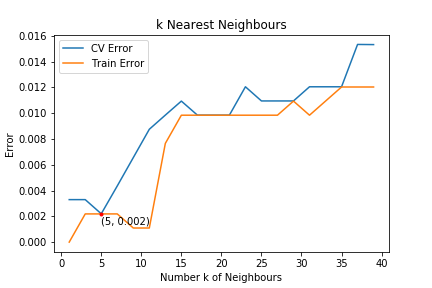
\includegraphics{Best K value - K-nearest Neighbours.png}

\subsection{Kernel Naive Bayes Classifier}

Let $\mathcal{C}_{k}$ be a class and let $\mathbf{x}$ our data vector.
As done before, we can apply Bayes' theorem to provide the \textit{a
	posteriori} probability of belonging to such class by stating \ref{eq:-13}.
Naive Bayes' classifier is based on the hypothesis that the attributes
of our data are conditionally independent, allowing us to rewrite
the conditional likelihood as 
\begin{equation}
\mathsf{p}\left(\mathbf{x}|\,\mathcal{C}_{k}\right)=\prod_{i=1}^{r}\mathsf{p}\left(x_{i}|\,\mathcal{C}_{k}\right).\label{eq:-14}
\end{equation}
This assumption, that is in fact \textit{naive}, does not usually
hurt too much as we are interested in picking the maximum probability
a\textit{ posteriori}. 

Naive Bayes is usually implemented by considering a probability density
function, that is fitted to the feature being taken into account.
However, we decided to model the conditional distribution with a more
complex kernel density estimation to allow for more parameter freedom.
As far as the prior are concerned, we decided to consider the relative
frequencies of the two classes.\\

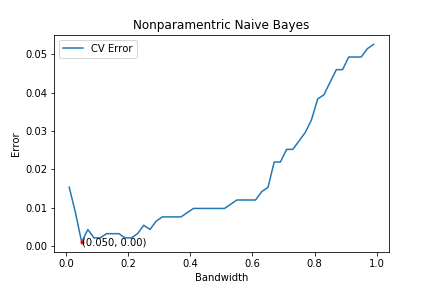
\includegraphics{Best Bandwidth - Naive Bayes.png}

Explain what are the three parameters that were optimized and their
effects on their respective classifiers. This will also require a
brief explanation of how each classifier works.\\
Explain the method by which the optimal values were found, noting
the differences between the errors and the importance of leaving out
a test set for the final evaluation\\
The report should show the error plots but no other plots are necessary\\

\section{Comparation}

\large McNemar's test
TALK ABOUT WHAT IS MCNEMAR TEST AND HOW IT WAS IMPLEMENTED AND USED\\
Estimate the true error for each classifier, compare the classifiers with McNemar's test and discuss which, if any, is better for this application\\


\section{Discussion and Conclusion}
This assignment aimed to help us understand the fundamental principles of three classifiers: Logistic Regression, K-nearest Neighbours and Naive Bayes. It also allowed us to understand and apply some data management techniques such as preprocessing data (Load, Shuffle, Split) and the process of Cross Validation. 
The first step on this assignment was to load and preprocessing the data from a file which held data from the UCI machine learning repository about bank notes authenticity. The goal of the three classifiers was to predict either a bank note was real of fake based on four features (Variance, Skewness, Curtosis, Entropy).
A test of performance of those classifiers was done to compare and eventually choose the best and to discuss if any is significantly better than the others. From the McNemar's tests we noticed that Logistic Regression and K-nearest Neighbours classifiers performances were similar. But in this particular case, Naive Bayes performance was way worse than the other two classifiers.
  

\section{Bibliography}
\begin{itemize}
\item ...\\
\end{itemize}

\end{document}